\begin{figure}[htbp]
\centering
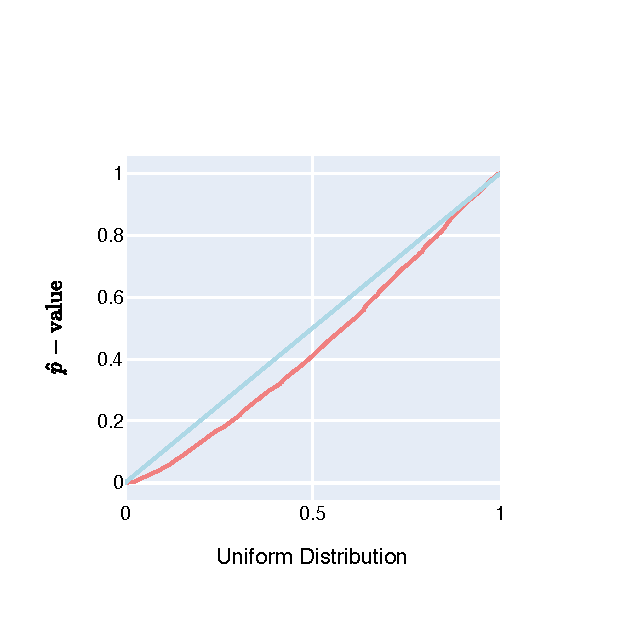
\includegraphics[width=0.6\textwidth]{figures/plots/drosophila/temp-EOP-QQ.pdf}
\caption{\textbf{The mutagenic process is equivalent between \textit{D. melanogaster} and \textit{D. simulans}.} The Quantile-Quantile plots compare the distribution of the temporal EOP between genes in \textit{D. melanogaster} and their ortholog in \textit{D. simulans} to  to the uniform distribution. The data point fall very close to the diagonal indication that the distribution is almost identical to what we would expect if the null was true. The plot shows 5942 third codon position CDS alignments from \textit{D. melanogaster}, \textit{D. simulans} and \textit{D. yakubra}. }
\label{fig:drosophila:temp-EOP-qq}
\end{figure}
